\documentclass[12pt]{beamer}
\newenvironment{ConCodigo}[1]
  {\begin{frame}[fragile,environment=ConCodigo]{#1}}
  {\end{frame}}
\graphicspath{{Imagenes/}{../Imagenes/}}
\usepackage[utf8]{inputenc}
\usepackage[spanish]{babel}
\usepackage{hyperref}
\usepackage{etex}
\reserveinserts{28}
\usepackage{amsmath}
\usepackage{amsthm}
\usepackage{mathtools}
\usepackage{multicol}
\usepackage{multirow}
\usepackage{tabulary}
%\usepackage{tabularx}
\usepackage{booktabs}
\usepackage{nccmath}
\usepackage{biblatex}
\usepackage{epstopdf}
\usepackage{graphicx}
\usepackage{siunitx}
\sisetup{scientific-notation=true}
%\usepackage{fontspec}
\usepackage{lmodern}
\usepackage{float}
\usepackage[format=hang, font=footnotesize, labelformat=parens]{caption}
\usepackage[autostyle,spanish=mexican]{csquotes}
\usepackage{standalone}
\usepackage{tikz}
\usepackage[siunitx]{circuitikz}
\usetikzlibrary{arrows,patterns,shapes}
\usetikzlibrary{decorations.markings}
\usetikzlibrary{arrows}
\usepackage{color}
%\usepackage{beton}
%\usepackage{euler}
%\usepackage[T1]{fontenc}
\usepackage[sfdefault]{roboto}  %% Option 'sfdefault' only if the base font of the document is to be sans serif
\usepackage[T1]{fontenc}
\renewcommand*\familydefault{\sfdefault}
\DeclareGraphicsExtensions{.pdf,.png,.jpg}
\usepackage{hyperref}
\renewcommand {\arraystretch}{1.5}
\newcommand{\python}{\texttt{python}}
\usefonttheme[onlymath]{serif}
\setbeamertemplate{navigation symbols}{}
\usetikzlibrary{patterns}
\usetikzlibrary{decorations.markings}
\tikzstyle{every picture}+=[remember picture,baseline]
%\tikzstyle{every node}+=[inner sep=0pt,anchor=base,
%minimum width=2.2cm,align=center,text depth=.15ex,outer sep=1.5pt]
%\tikzstyle{every path}+=[thick, rounded corners]
\setbeamertemplate{caption}[numbered]
\newcommand{\ptm}{\fontfamily{ptm}\selectfont}
%Se usa la plantilla Warsaw modificada con spruce
\mode<presentation>
{
  \usetheme{Warsaw}
  \setbeamertemplate{headline}{}
  \useoutertheme{default}
  \usecolortheme{beaver}
  \setbeamercovered{invisible}
}
\AtBeginSection[]
{
\begin{frame}<beamer>{Contenido}
\normalfont\mdseries
\tableofcontents[currentsection]
\end{frame}
}

\usepackage{listings}
\lstset{ %
language=Python,                % choose the language of the code
basicstyle=\small,       % the size of the fonts that are used for the code
numbers=left,                   % where to put the line-numbers
numberstyle=\small,      % the size of the fonts that are used for the line-numbers
stepnumber=1,                   % the step between two line-numbers. If it is 1 each line will be numbered
numbersep=5pt,                  % how far the line-numbers are from the code
backgroundcolor=\color{white},  % choose the background color. You must add \usepackage{color}
showspaces=false,               % show spaces adding particular underscores
showstringspaces=false,         % underline spaces within strings
showtabs=false,                 % show tabs within strings adding particular underscores
frame=single,   		% adds a frame around the code
tabsize=2,  		% sets default tabsize to 2 spaces
captionpos=b,   		% sets the caption-position to bottom
breaklines=true,    	% sets automatic line breaking
breakatwhitespace=false,    % sets if automatic breaks should only happen at whitespace
escapeinside={\%},          % if you want to add a comment within your code
stringstyle =\color{magenta},
keywordstyle = \color{blue},
commentstyle = \color{green},
identifierstyle = \color{red}
}
\begin{document}
\title{Examen 2 - Operaciones matemáticas básicas}
\subtitle{Solución}
\author{M. en C. Gustavo Contreras Mayén}
\maketitle
\fontsize{14}{14}\selectfont
\spanishdecimal{.}
\begin{frame}{Contenido}
\tableofcontents[pausesections]
\end{frame}
\begin{frame}[fragile]
\frametitle{Problema 1}
Dados los puntos
	\begin{table}[H]
		\centering 
		\begin{large}
			\begin{tabulary}{15cm}{c | c | c | c  }\normalsize
				$x$ & $-1.2$ & $0.3$ & $1.1$ \\
				\midrule
				$y$ & $-5.76$ & $-5.61$ & $-3.69$
			\end{tabulary}
		\end{large}
	\end{table}
	Calcula $y$ en $x=0$ usando: a) el método de Neville y b) el método de Lagrange.
	\\
	\medskip
	\visible<2->{\textcolor{red}{La raíz en ambos métodos, vale $-6.0$}}
\end{frame}
\begin{frame}
\frametitle{Problema 2}
Encontrar la raíz de $y(x)$ a partir de los siguientes datos:
	\begin{table}[H]
		\centering 
		\begin{large}
			\begin{tabulary}{15cm}{c | c | c | c | c | c | c | c }
				$x$ & $0$ & $0.5$ & $1$ & $1.5$ & $2$ & $2.5$ & $3$ \\
				\midrule
				$y$ & $1.8421$ & $2.4694$ & $2.4921$ & $1.9047$ & $0.8509$ & $-0.4112$ & $-1.5727$ 
			\end{tabulary}
		\end{large}	
	\end{table}
	Usando la interpolación de Lagrange sobre a) tres puntos, y b) sobre cuatro puntos vecinos más cercanos.
%	\visible<2->{\textcolor{red}{El valor de la raíz es: 2.3397}}
\end{frame}
\begin{frame}
\frametitle{Resultado}
\begin{figure}
	\centering
	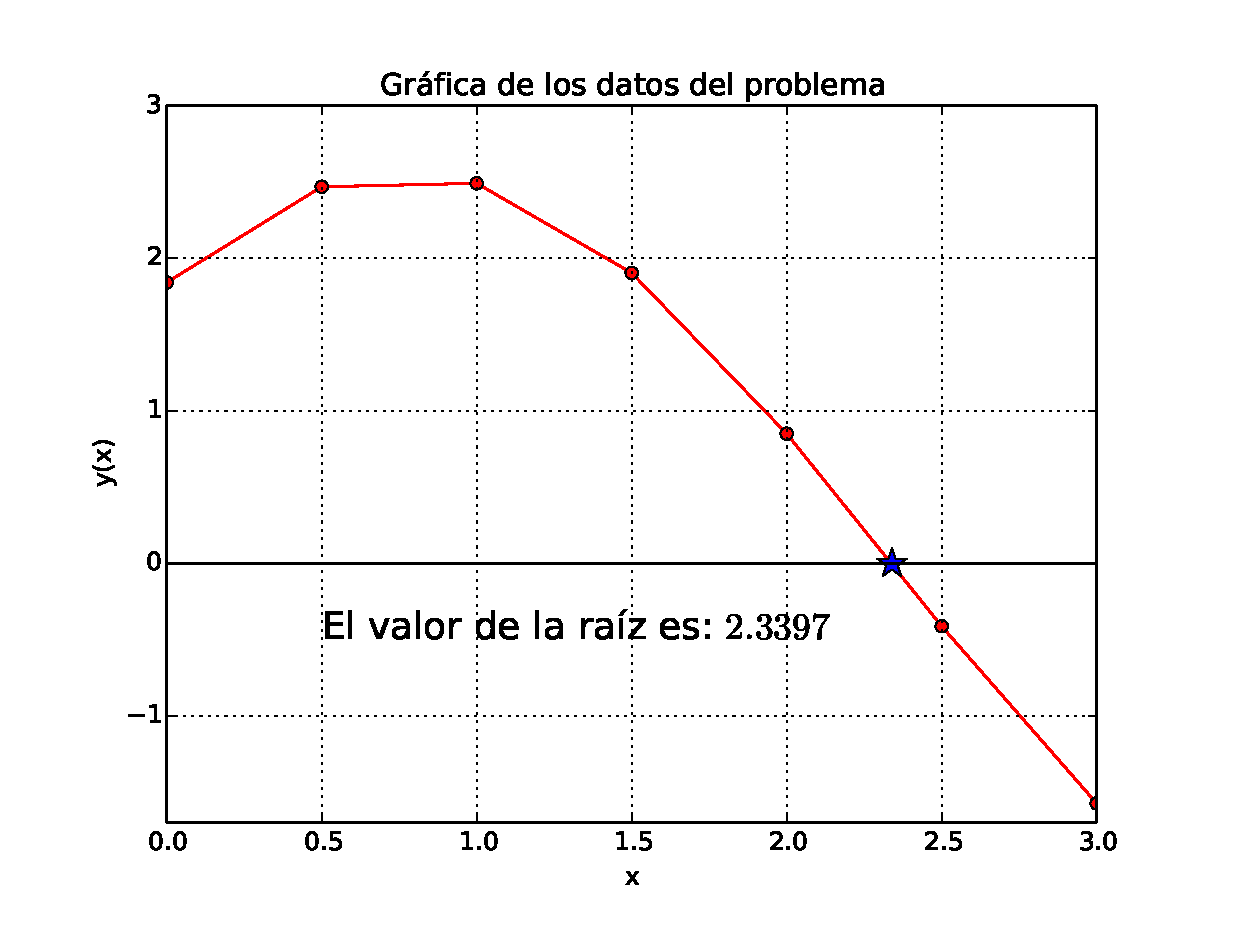
\includegraphics[scale=0.5]{Imagenes/Problema2_01.eps} 
\end{figure}
\end{frame}
\begin{frame}
\frametitle{Problema 3}
La función $y(x)$ del problema anterior, tiene un máximo en $x=0.7679$. Calcular el valor máximo con el método de interpolación de Neville usando cuatro puntos vecinos.
\\
\bigskip
%\visible<2->{\textcolor{red}{El valor máximo de la función es: 2.5568}}
\end{frame}
\begin{frame}
\frametitle{Resultado}
\begin{figure}
	\centering
	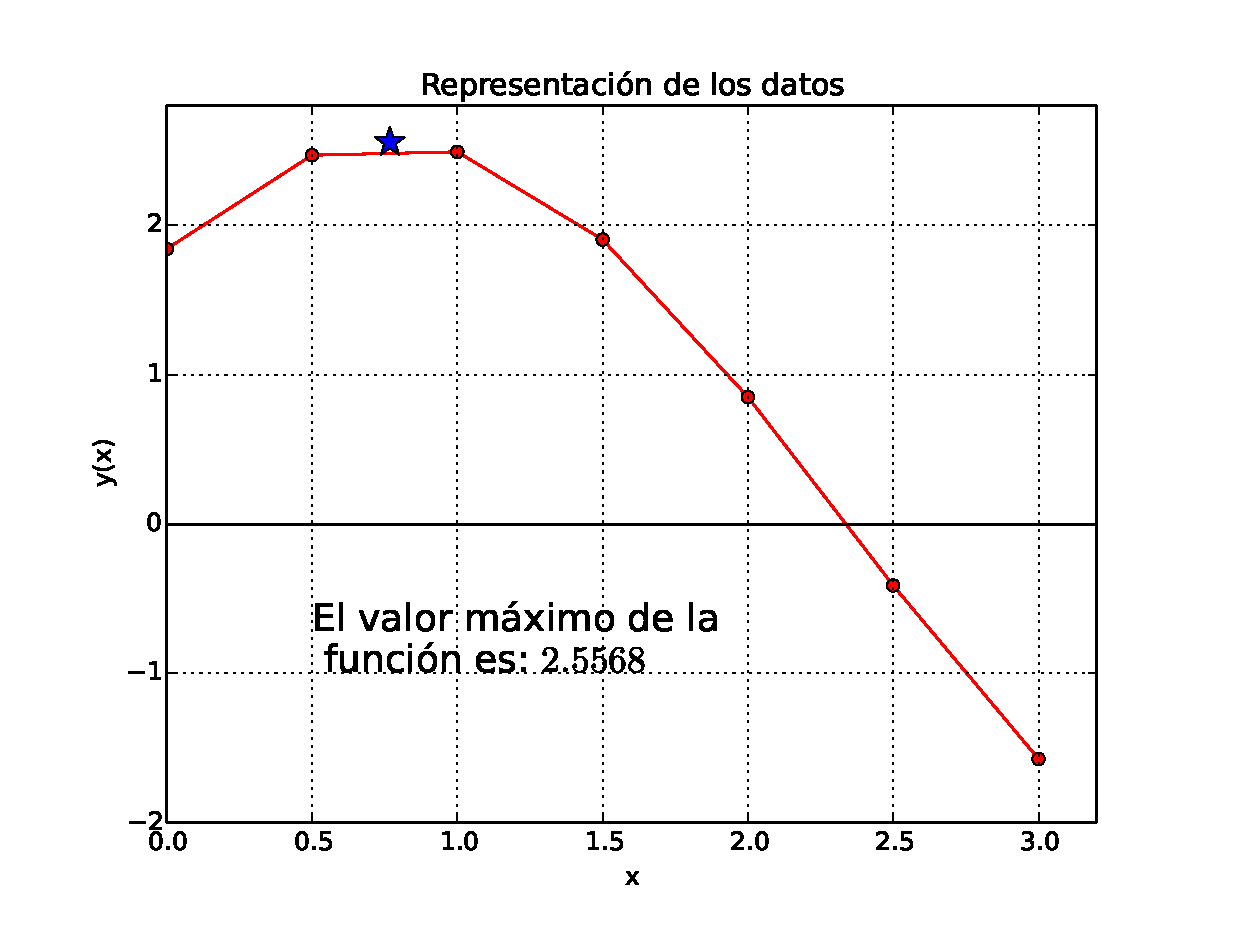
\includegraphics[scale=0.5]{Imagenes/Problema3_01.eps} 
\end{figure}
\end{frame}
\begin{frame}
\frametitle{Problema 4}
La viscosidad cinemática $\mu_{k}$ del agua varía con la temperatura $T$ de la siguiente manera:
	\begin{table}[H]
		\centering
		\fontsize{12}{12}\selectfont
				\begin{tabulary}{15cm}{c | c | c | c | c | c | c | c }
					$T(^\circ C)$ & $0$ & $21.1$ & $37.8$ & $54.4$ & $71.1$ & $87.8$ & $100$ \\
					\midrule
					$\mu_{k} (10^{-3}m^{2}/s)$ & $1.79$ & $1.13$ & $0.696$ & $0.519$ & $0.338$ & $0.321$ & $0.296$ 
				\end{tabulary}
	\end{table}
	Interpolar $\mu_{k}$ para $T= 10^{\circ},30^{\circ},60^{\circ}$ y $90^{\circ}$.
\end{frame}
\begin{frame}
\frametitle{Solución Problema 4}
\begin{figure}
	\centering
	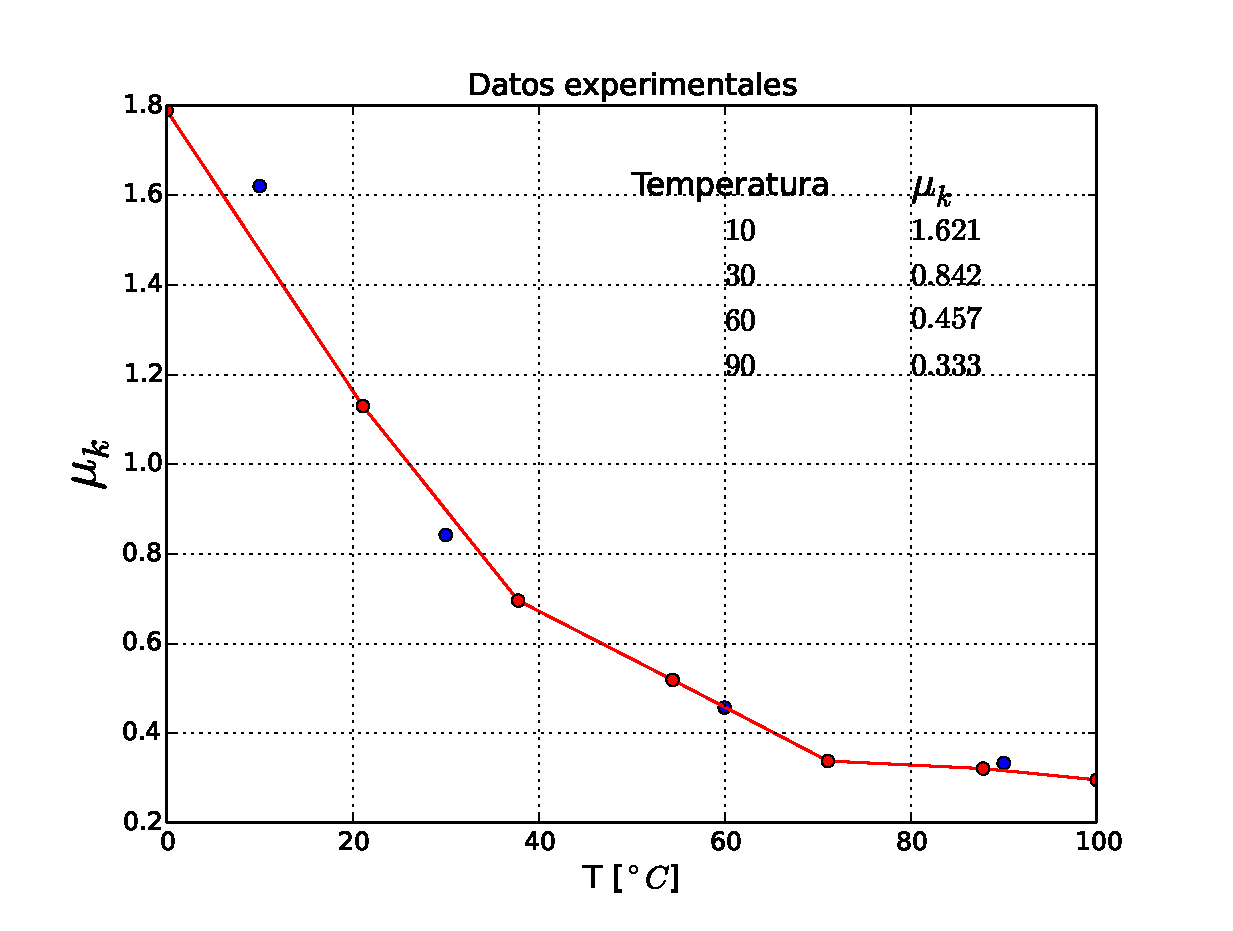
\includegraphics[scale=0.5]{Imagenes/Problema4_01.eps} 
\end{figure}
\end{frame}
\begin{frame}
\frametitle{Problema 5}
La siguiente tabla muesta como la densidad relativa $\rho$ del aire varía con la altitud $h$. Calcula la densidad relativa del aire en $10.5$ km.
	\begin{table}[H]
		\centering 
		\fontsize{12}{12}\selectfont
			\begin{tabulary}{15cm}{c | c | c | c | c | c | c | c }
				$h(km)$ & $0$ & $1.525$ & $3.050$ & $4.575$ & $6.10$ & $7.625$ & $9.150$ \\
				\midrule
				$\rho$ & $1$ & $0.8617$ & $0.7385$ & $0.6292$ & $0.5328$ & $0.4481$ & $0.3741$ 
			\end{tabulary}
	\end{table}
%	\visible<2->{\textcolor{red}{La densidad del aire en 10.5 km es de 0.3177}}
\end{frame}
\begin{frame}
\frametitle{Solución Problema 5}
\begin{figure}
	\centering
	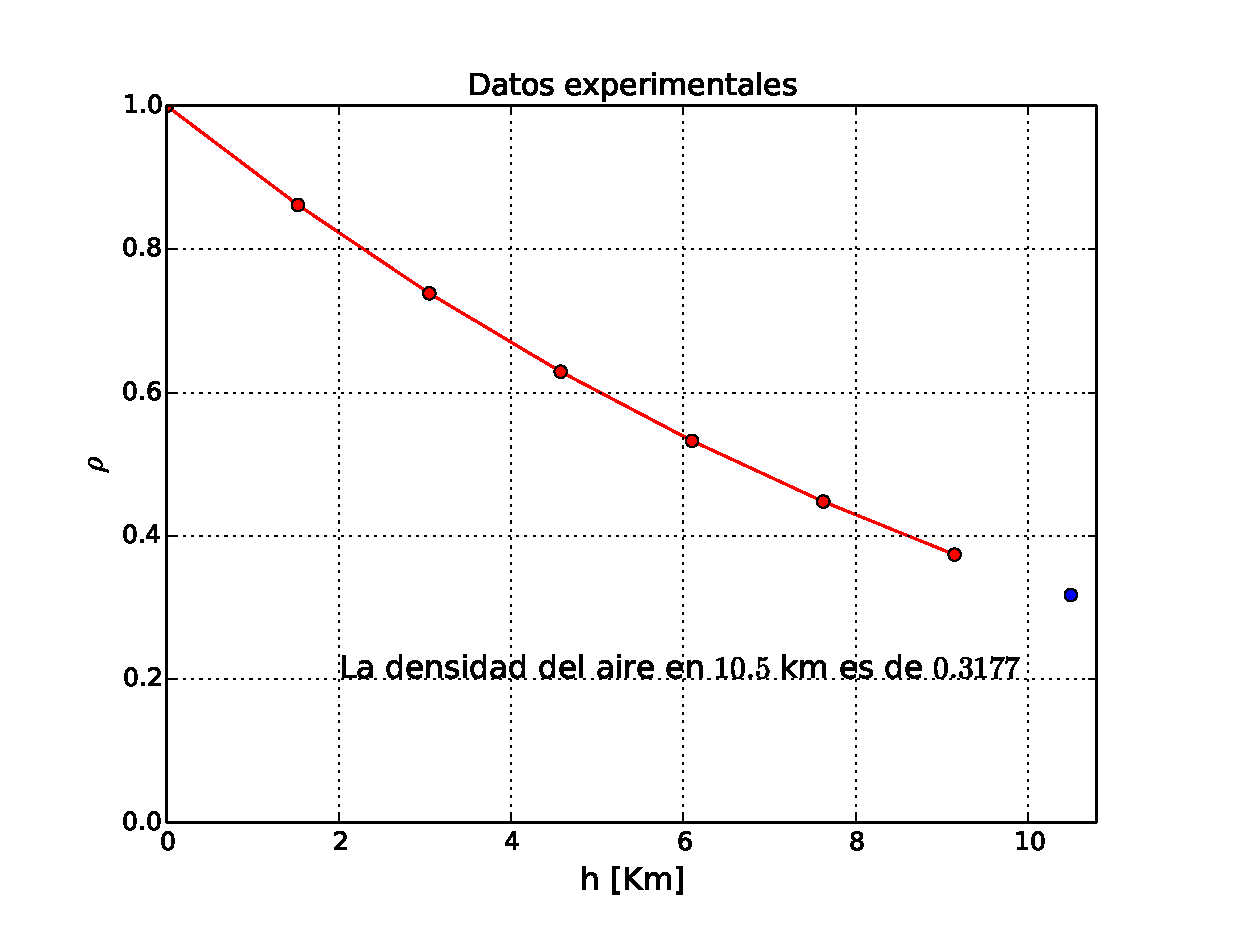
\includegraphics[scale=0.5]{Imagenes/Problema5_01.eps} 
\end{figure}
\end{frame}
\begin{frame}
\frametitle{Problema 6}
Encuentra todas las raíces positivas de las siguientes ecuaciones mediante el método de bisección, con una tolerancia de 0.001.
	\begin{enumerate}\label{grupo1}
	\renewcommand{\arraystretch}{1.5}
		\item $\tan(x) - x + 1 = 0; \hspace{1cm} 0 < x < 3\pi$
		\item $\sin(x) - 0.3 \exp(x) = 0; \hspace{1cm} x > 0$
		\item $-x^{3} + x + 1 = 0$
		\item $16x^{5} - 20x^{3} + x^{2} + 5x - 0.5 = 0$
	\end{enumerate}
\end{frame}
\begin{frame}
\frametitle{Inciso a) $\tan(x) - x + 1 = 0; \hspace{1cm} 0 < x < 3\pi$}
\begin{figure}
	\centering
	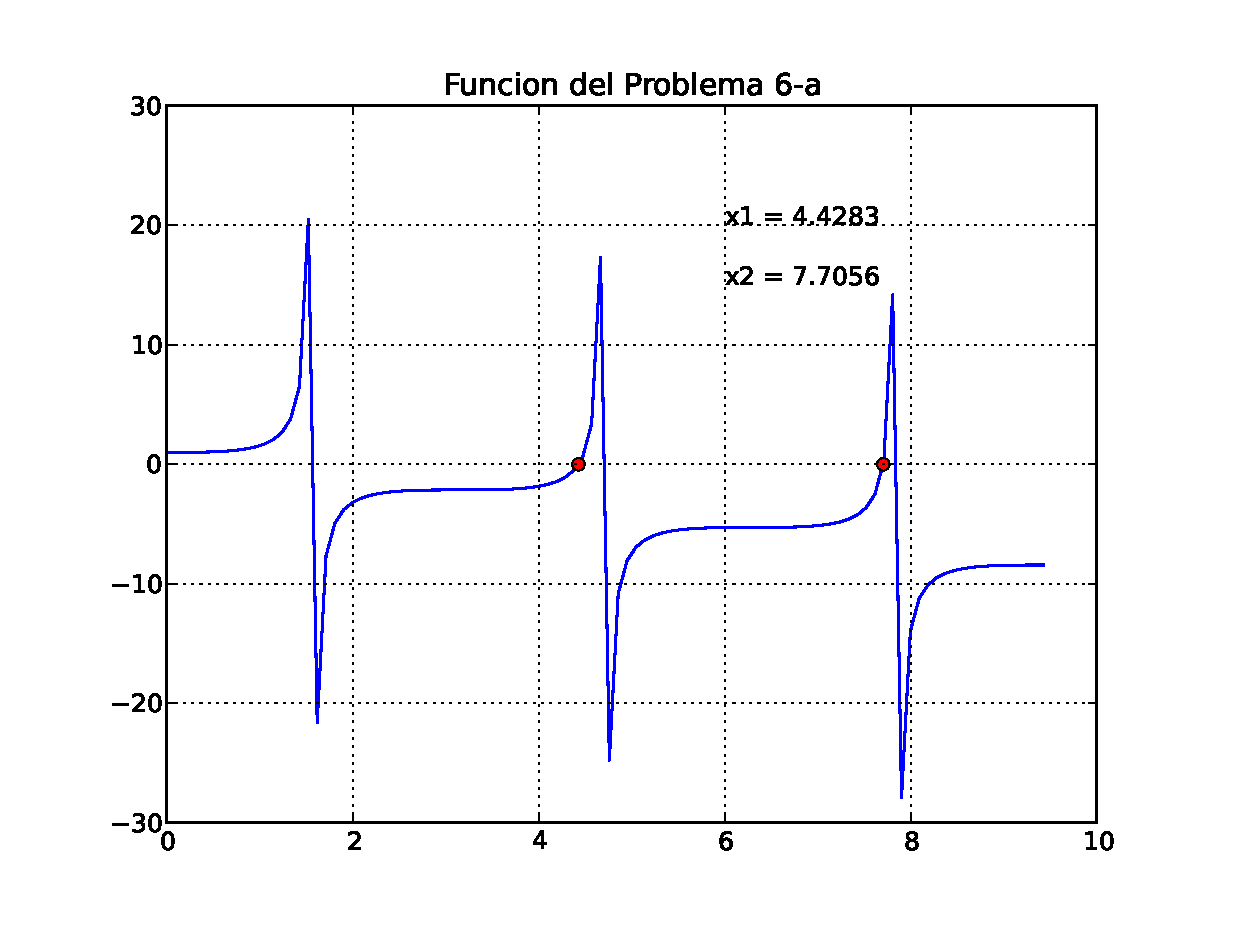
\includegraphics[scale=0.5]{Grafica6_a.eps}
\end{figure}
\end{frame}
\begin{frame}
\frametitle{Inciso b) $\sin(x) - 0.3 \exp(x) = 0; \hspace{1cm} x > 0$}
\begin{figure}
	\centering
	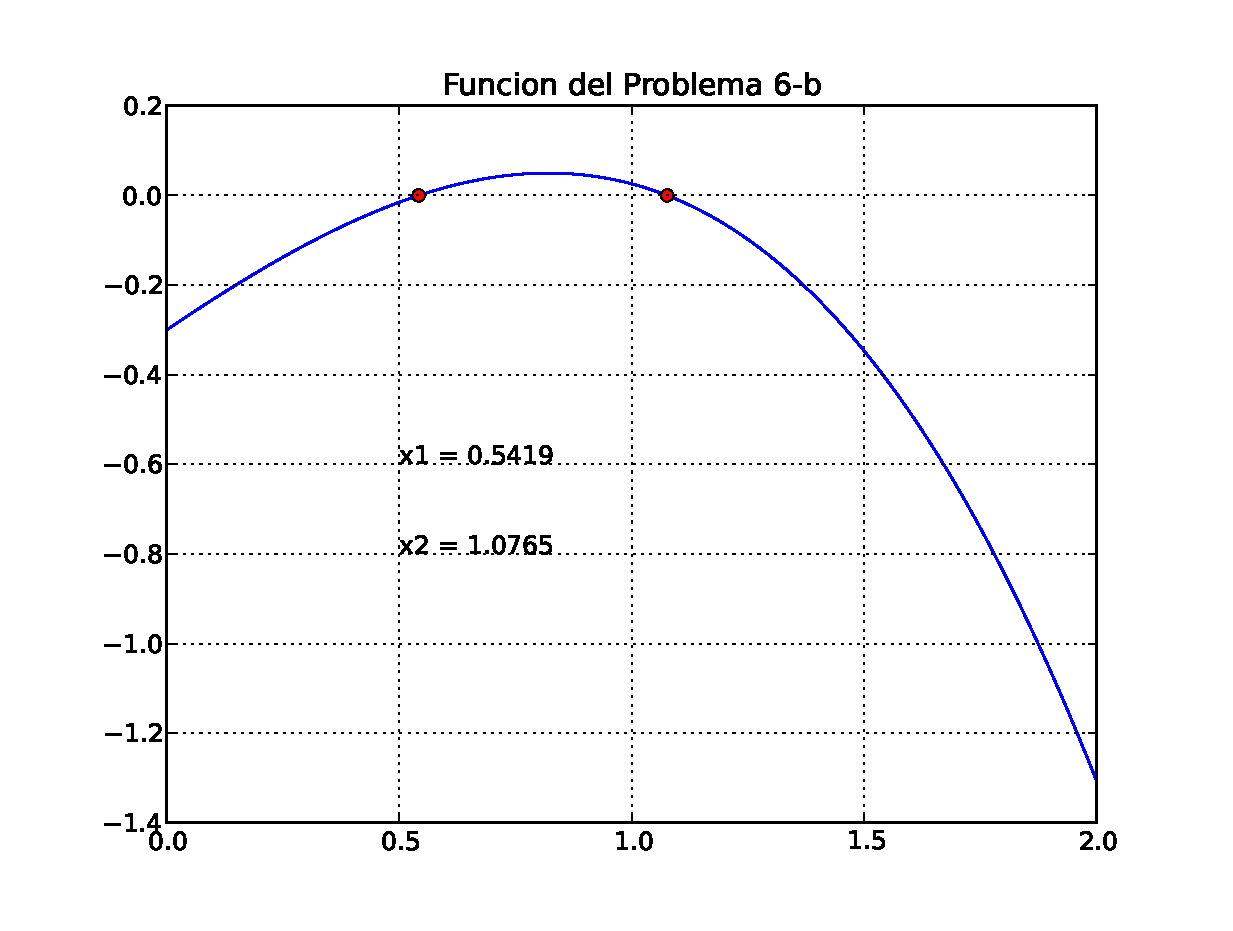
\includegraphics[scale=0.5]{Grafica6_b.eps}
\end{figure}
\end{frame}
\begin{frame}
\frametitle{Inciso c)$-x^{3} + x + 1 = 0$}
\begin{figure}
	\centering
	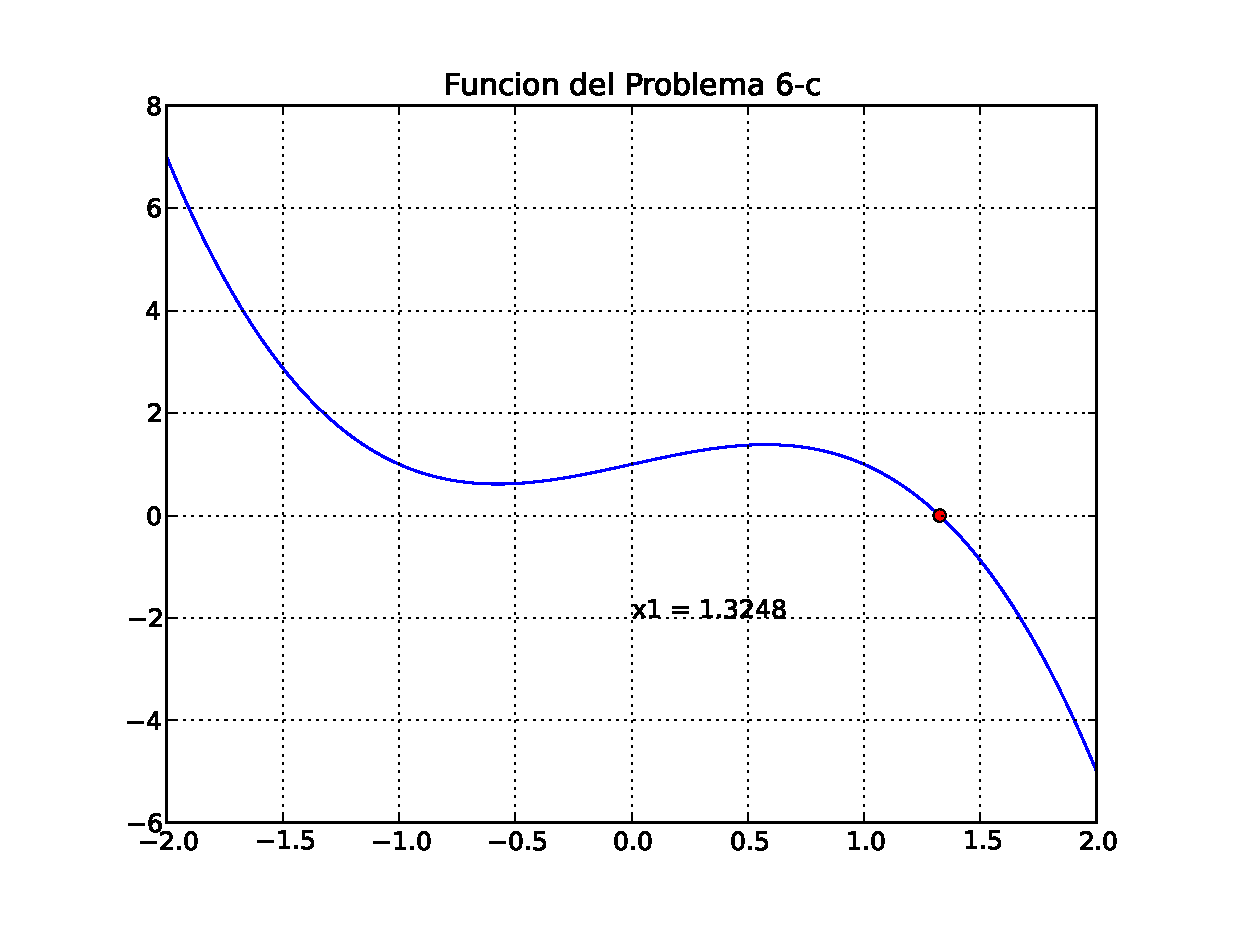
\includegraphics[scale=0.5]{Grafica6_c.eps}
\end{figure}
\end{frame}
\begin{frame}
\frametitle{Inciso d)$16x^{5} - 20x^{3} + x^{2} + 5x - 0.5 = 0$}
\begin{figure}
	\centering
	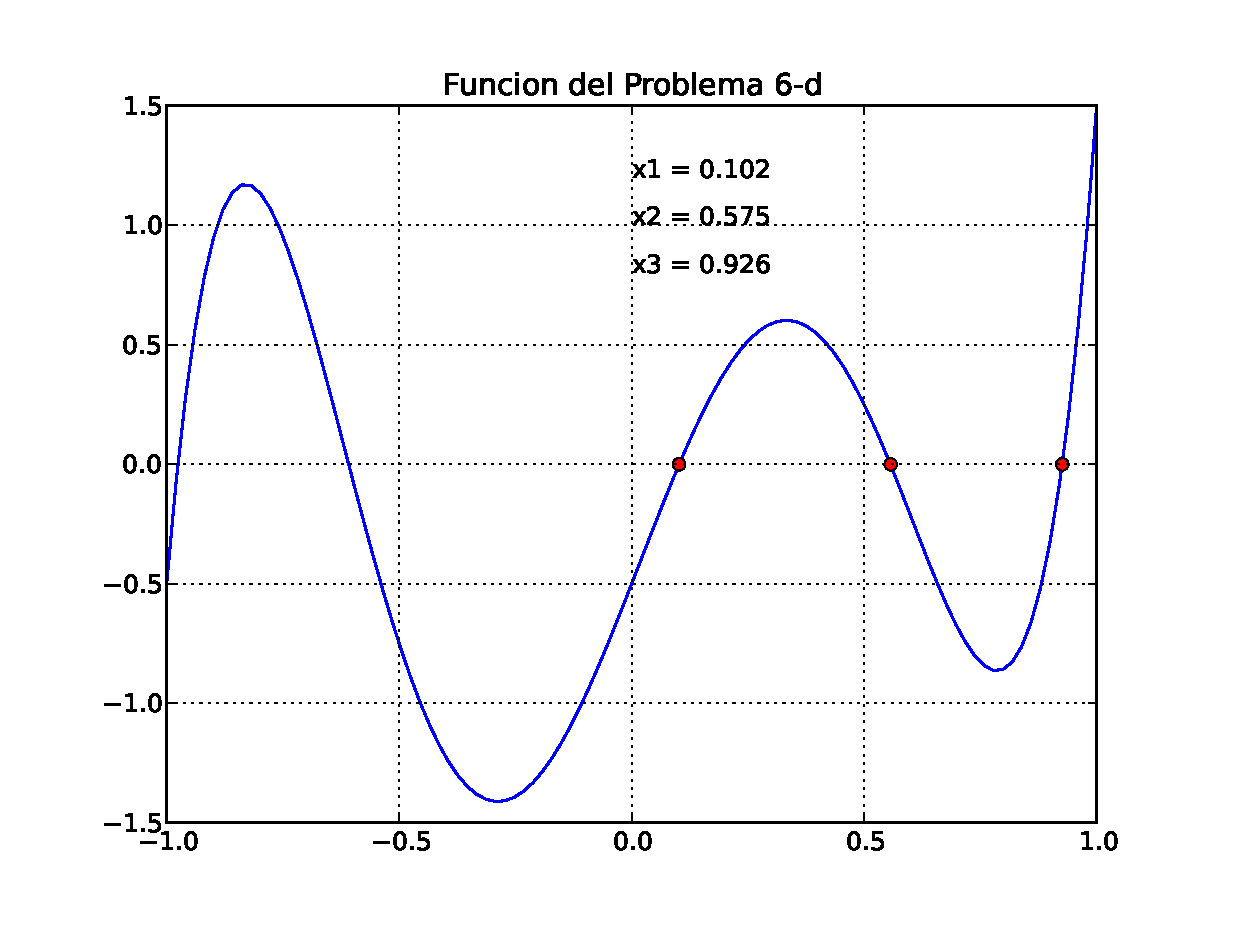
\includegraphics[scale=0.5]{Grafica6_d.eps}
\end{figure}
\end{frame}
\begin{frame}
\frametitle{Problema 7}
Determina las raíces de las siguientes ecuaciones mediante el método de la falsa posición modificada:
	\begin{enumerate}
		\renewcommand{\arraystretch}{1.5}
		\item $f(x) = 0.5\exp(\frac{x}{3})- \sin(x); \hspace{1cm} x > 0$
		\item $g(x) = \log(1 + x) - x^{2}$
		\item $f(x) = \exp(x) - 5x^{2}$
		\item $h(x) = x^{3} + 2x - 1 = 0$
		\item $f(x) = \sqrt{x+2}$
	\end{enumerate}
\end{frame}
\begin{frame}
\frametitle{Inciso a) $f(x) = 0.5\exp(\frac{x}{3})- \sin(x); \hspace{1cm} x > 0$}
\begin{figure}
	\centering
	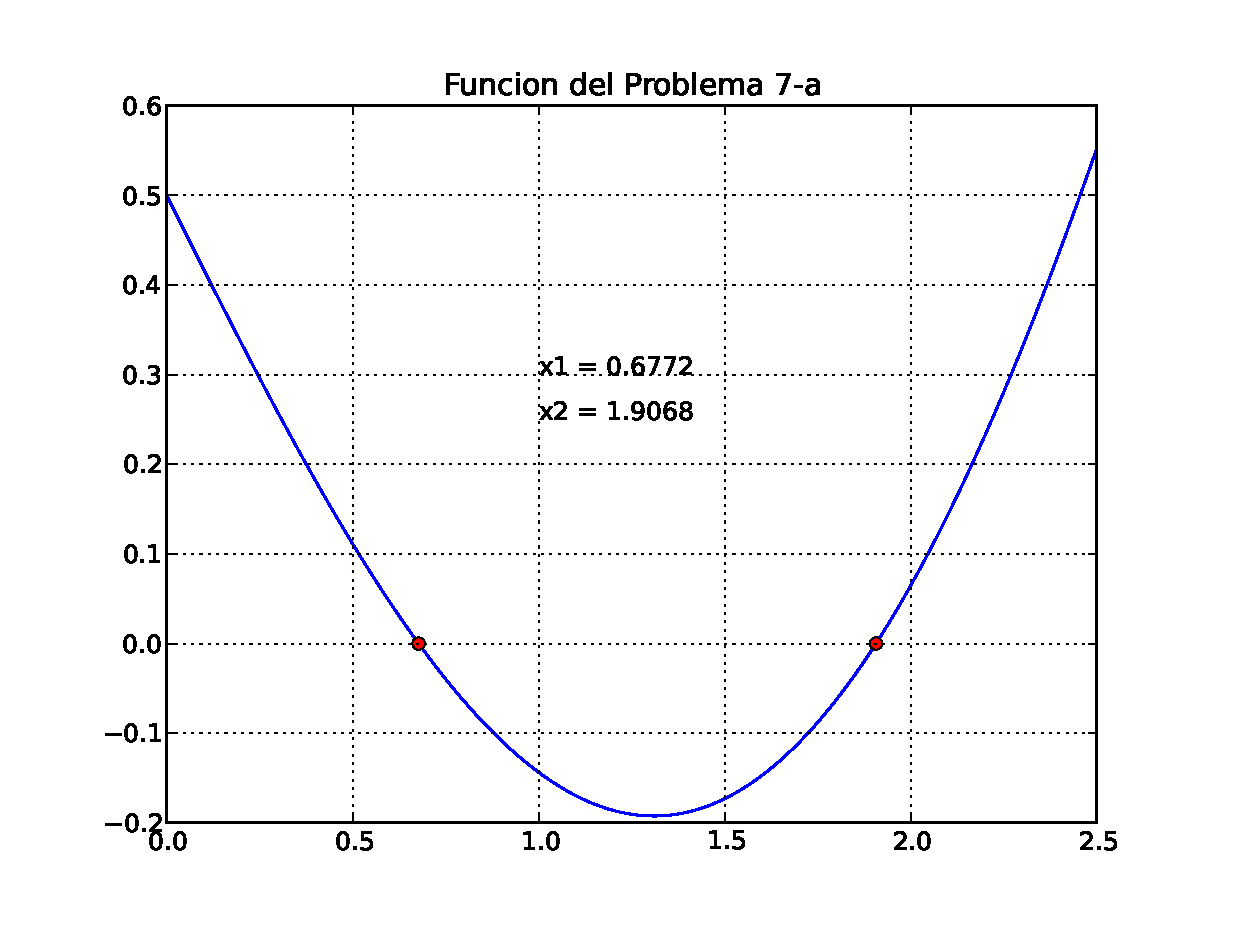
\includegraphics[scale=0.4]{Grafica7_a1.eps}
\end{figure}
\end{frame}
\begin{frame}
\frametitle{Inciso b) $g(x) = \log(1 + x) - x^{2}$}
\begin{figure}
	\centering
	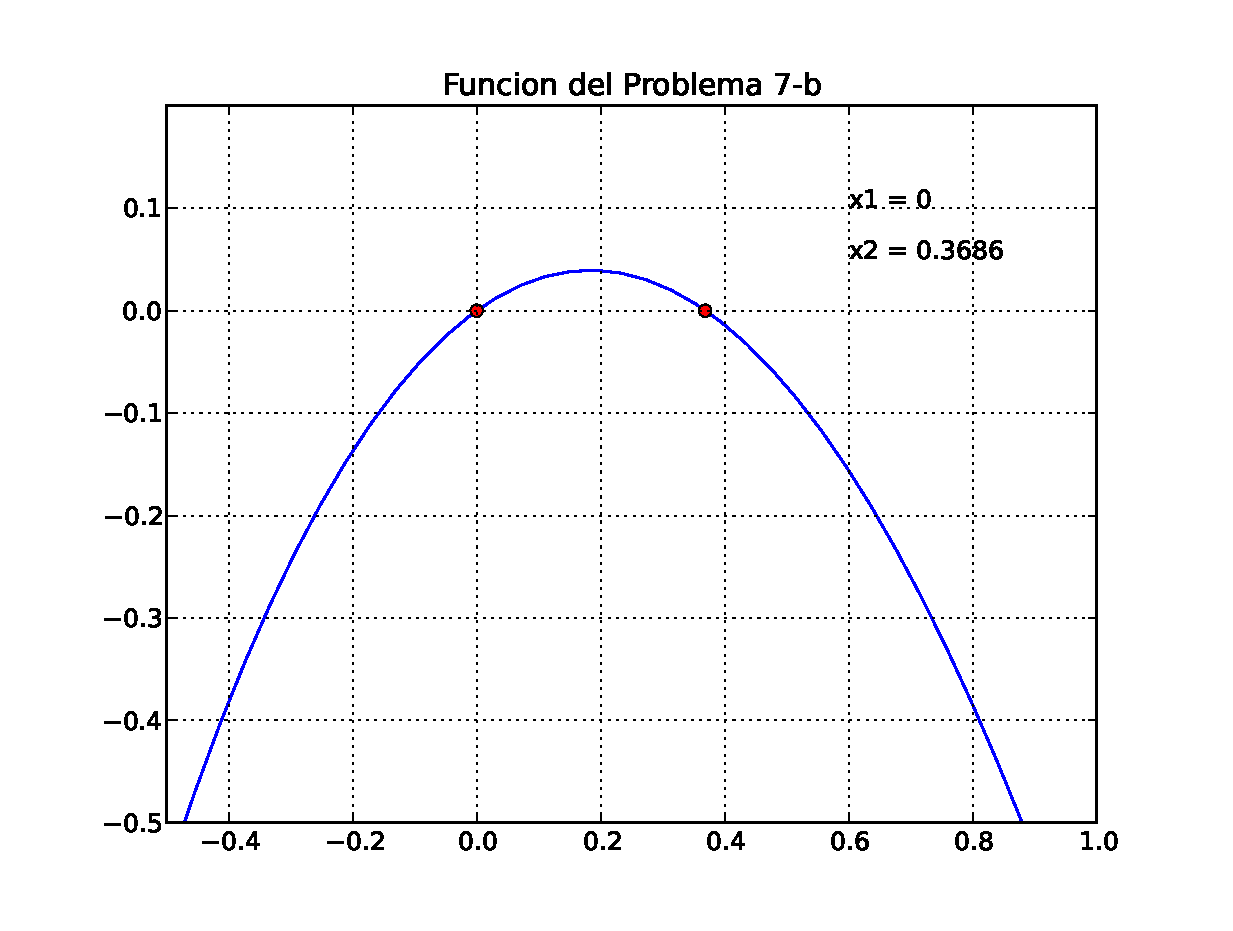
\includegraphics[scale=0.4]{Grafica7_b.eps}
\end{figure}
\end{frame}
\begin{frame}
\frametitle{Inciso c) $f(x) = \exp(x) - 5x^{2}$}
\begin{figure}
	\centering
	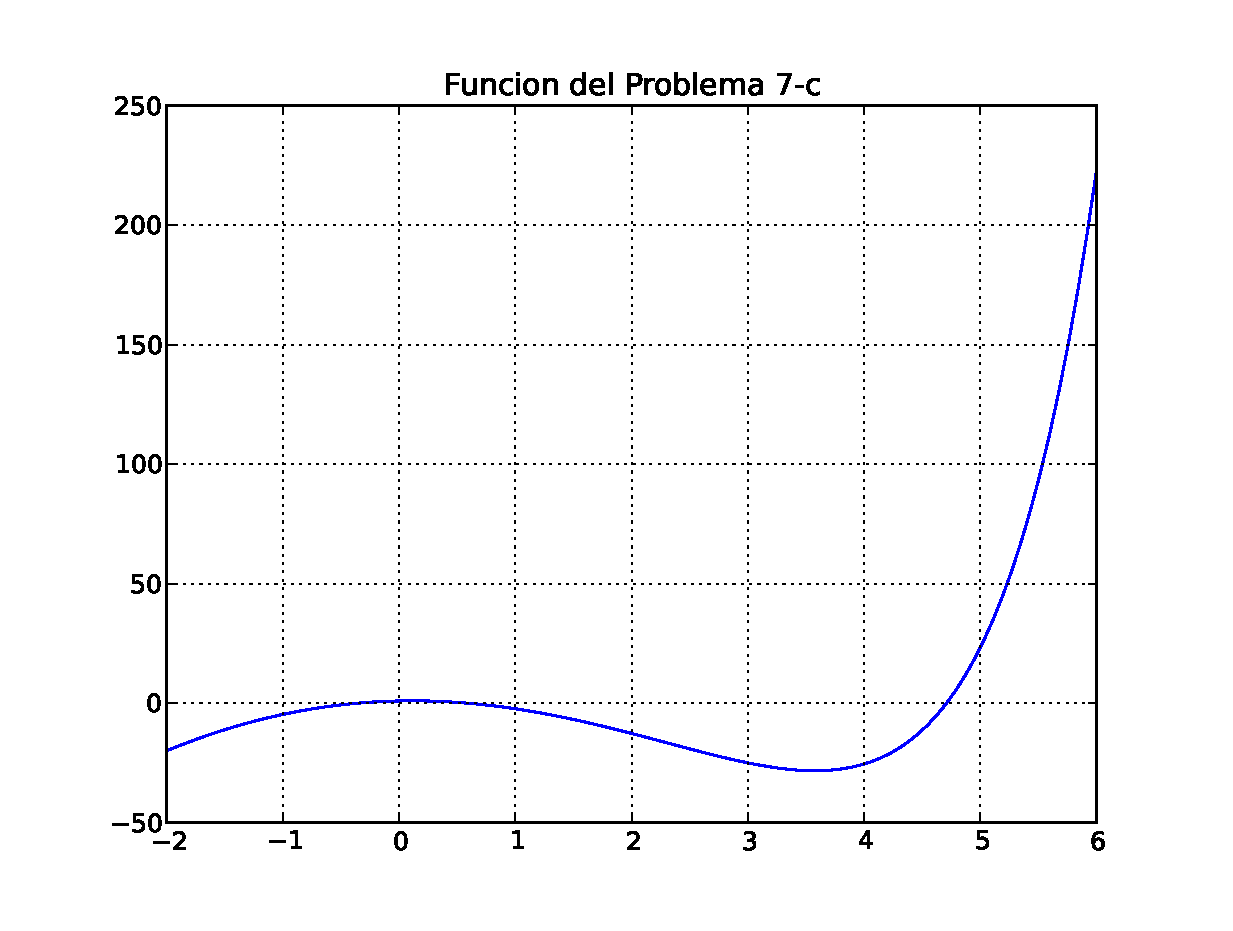
\includegraphics[scale=0.4]{Grafica7_c1.eps}<1>
	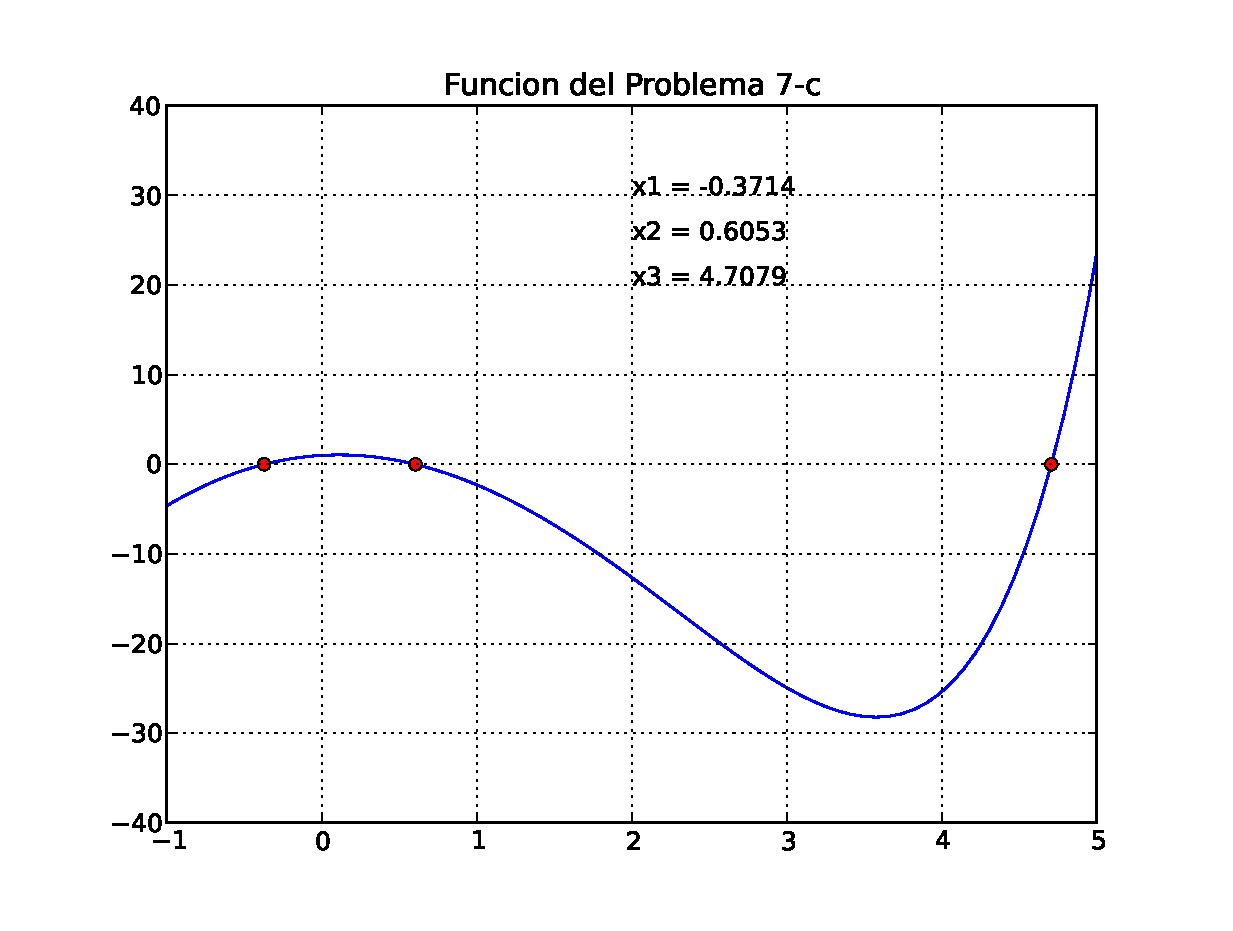
\includegraphics[scale=0.4]{Grafica7_c2.eps}<2>
\end{figure}
\end{frame}
\begin{frame}
\frametitle{Inciso d) $h(x) = x^{3} + 2x - 1 = 0$}
\begin{figure}
	\centering
	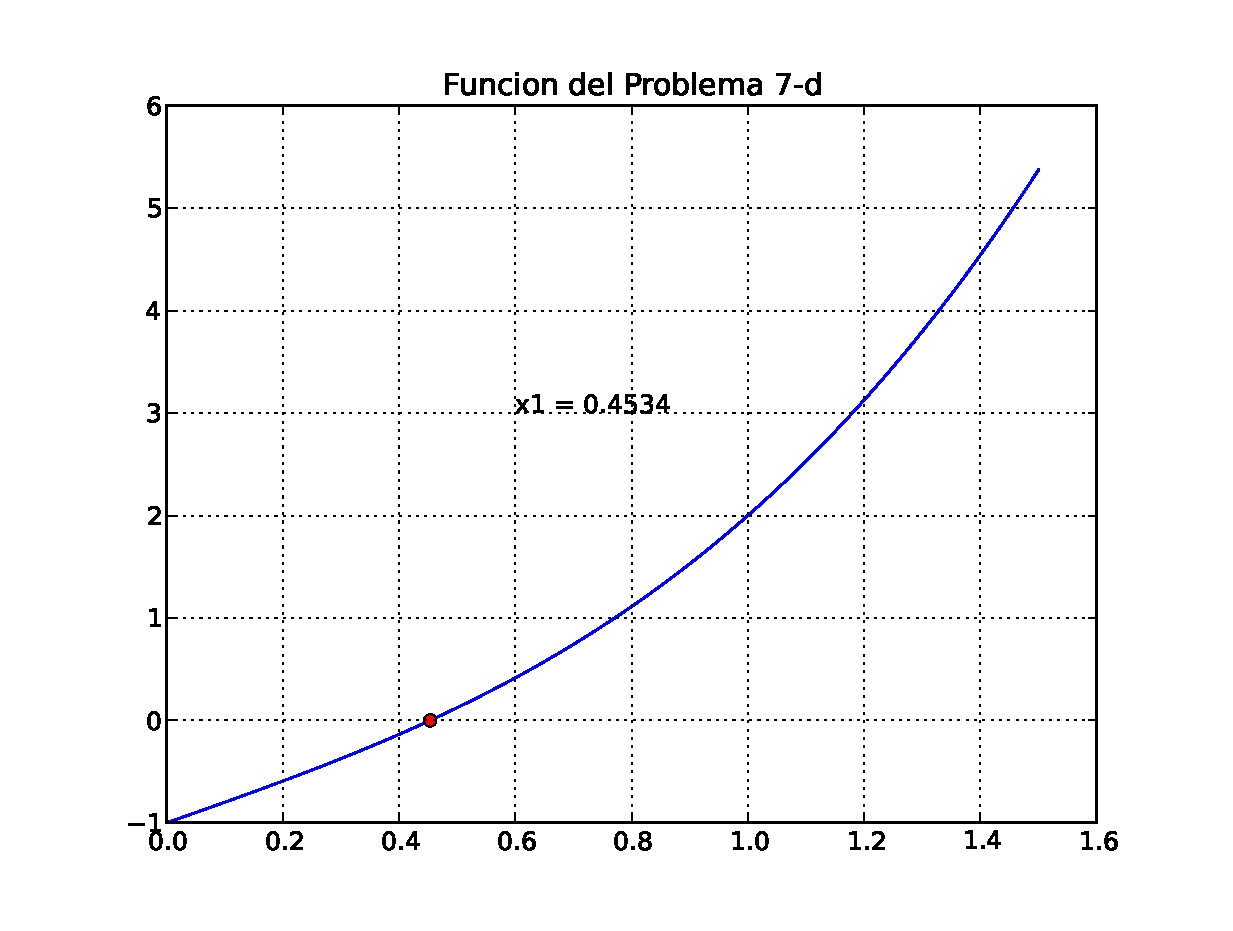
\includegraphics[scale=0.4]{Grafica7_d.eps}
\end{figure}
\end{frame}
\begin{frame}
\frametitle{Inciso e)$f(x) = \sqrt{x+2}$}
\begin{figure}
	\centering
	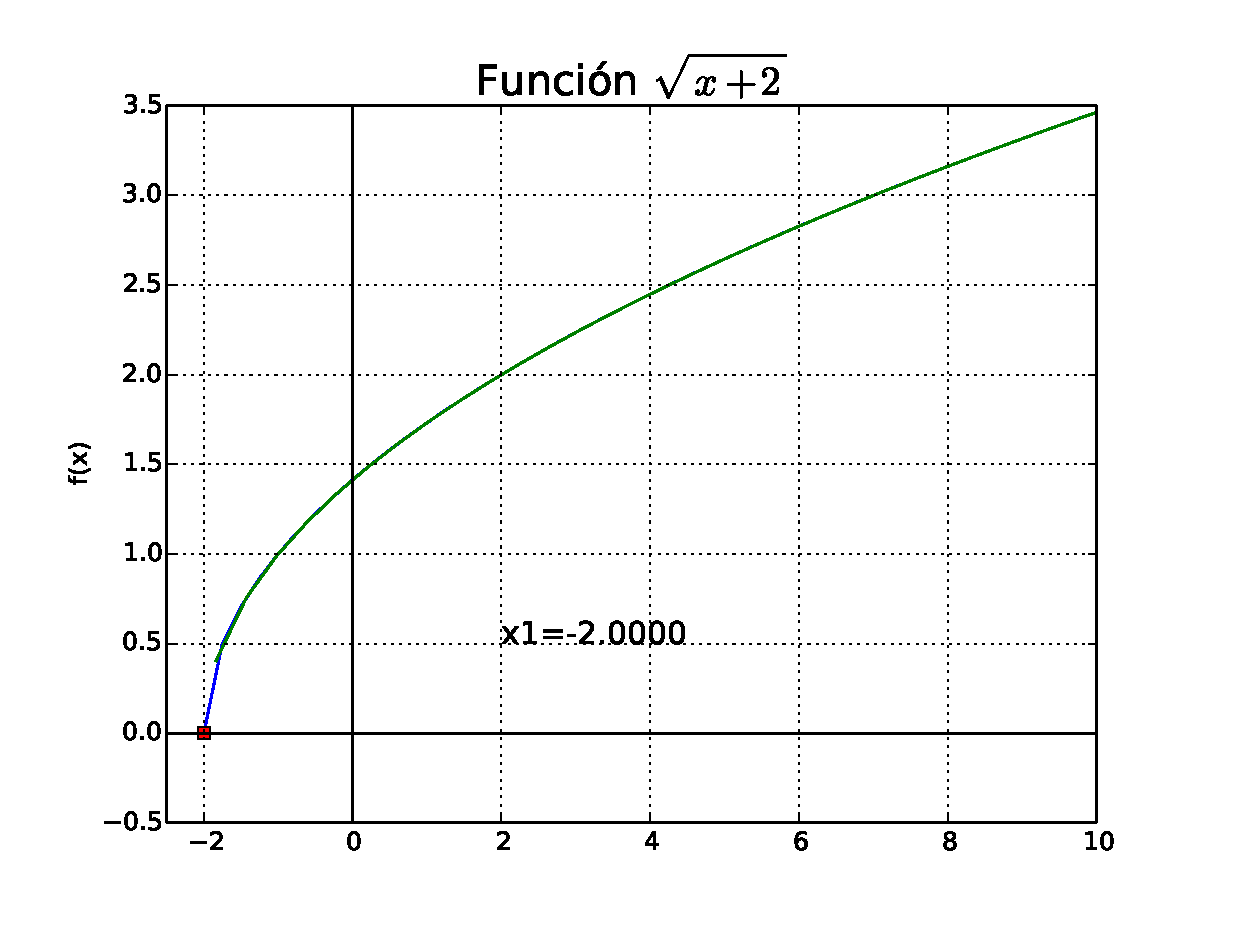
\includegraphics[scale=0.4]{Grafica7_e.eps}
\end{figure}
\end{frame}
\begin{frame}
\frametitle{Problema 8}
Dado que ya conocen las raíces de las funciones, esperaríamos que reportaran un valor casi idéntico, y hasta con un error relativo.
\end{frame}
\begin{frame}
\frametitle{Problema 9}
Identifica el intervalo para las raíces de las siguientes ecuaciones y calcula despúes las raíces mediante el método de la secante, con una tolerancia de $0.001$:
	\begin{enumerate}
		\item $0.1 x^{3} - 5 x^{2} - x + 4 + \exp(-x) = 0 $
		\item $\ln(x) -0.2 x^{2} + 1 = 0$
		\item $x + \dfrac{1}{(x+3)x}= 0$
	\end{enumerate}
\end{frame}
\begin{frame}
\frametitle{Inciso a)$0.1 x^{3} - 5 x^{2} - x + 4 + \exp(-x) = 0 $}
\begin{figure}
	\centering
	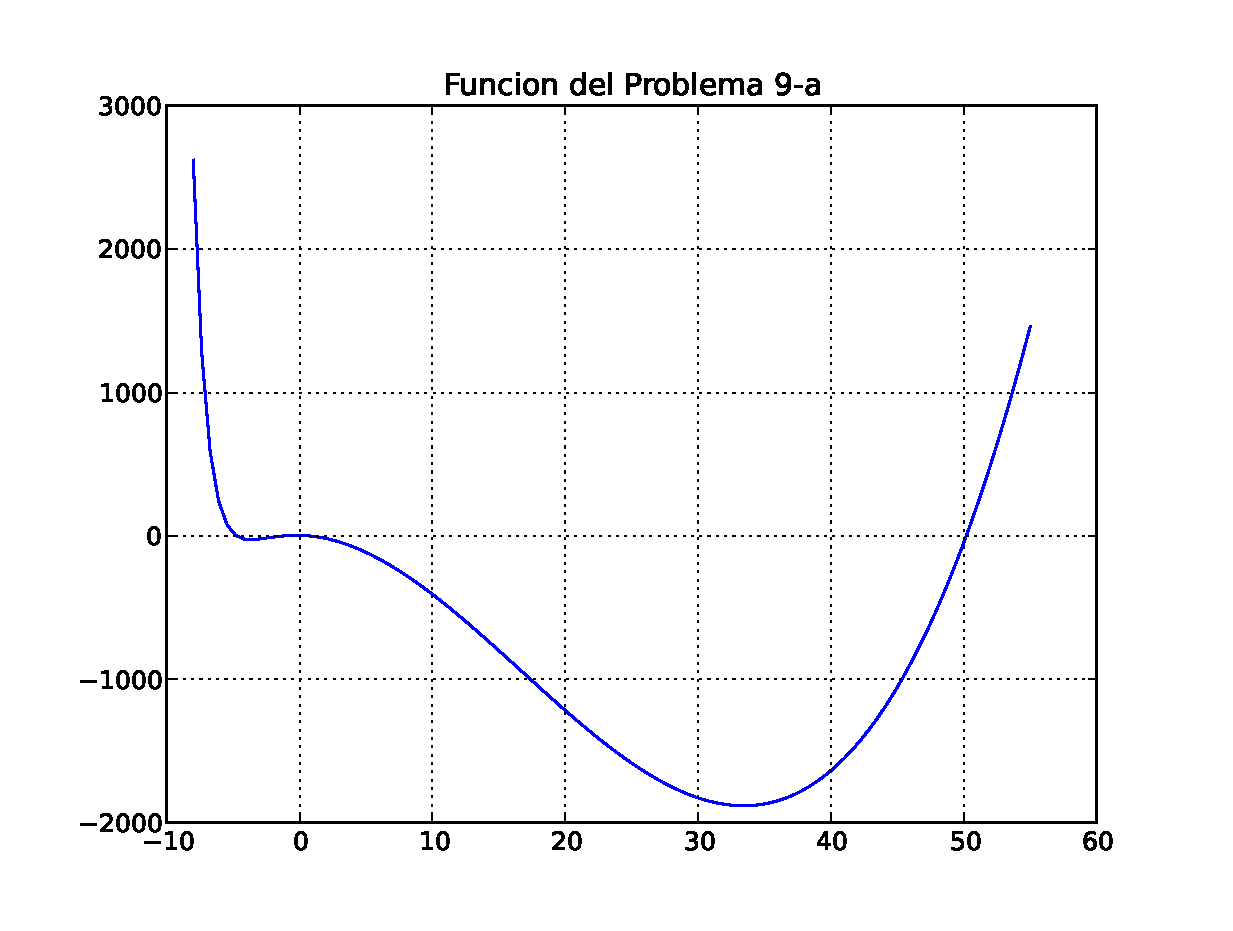
\includegraphics[scale=0.4]{Grafica9_a1.eps}<1> 
	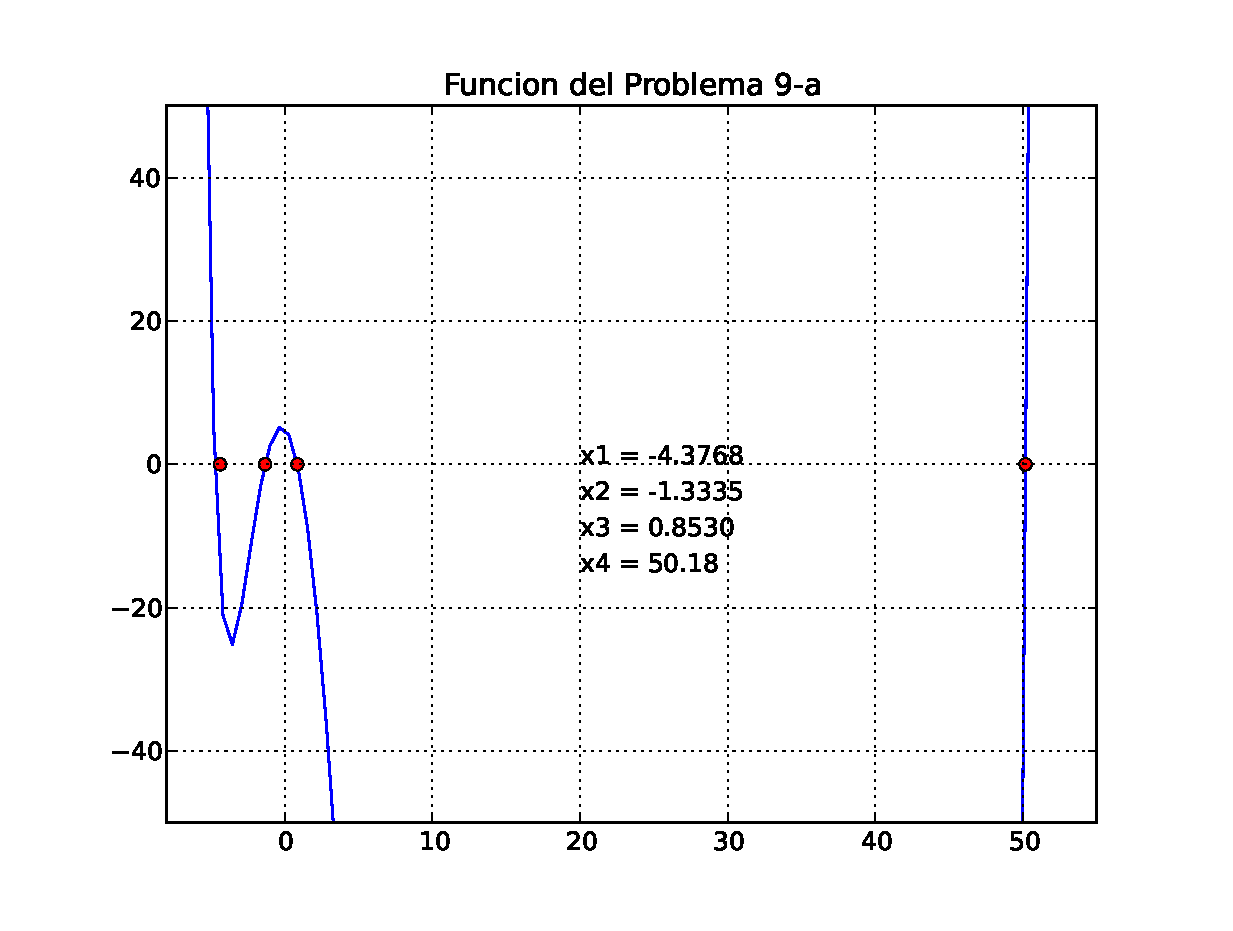
\includegraphics[scale=0.4]{Grafica9_a2.eps}<2>
\end{figure}
\end{frame}
\begin{frame}
\frametitle{Inciso b)}
\begin{figure}
	\centering
	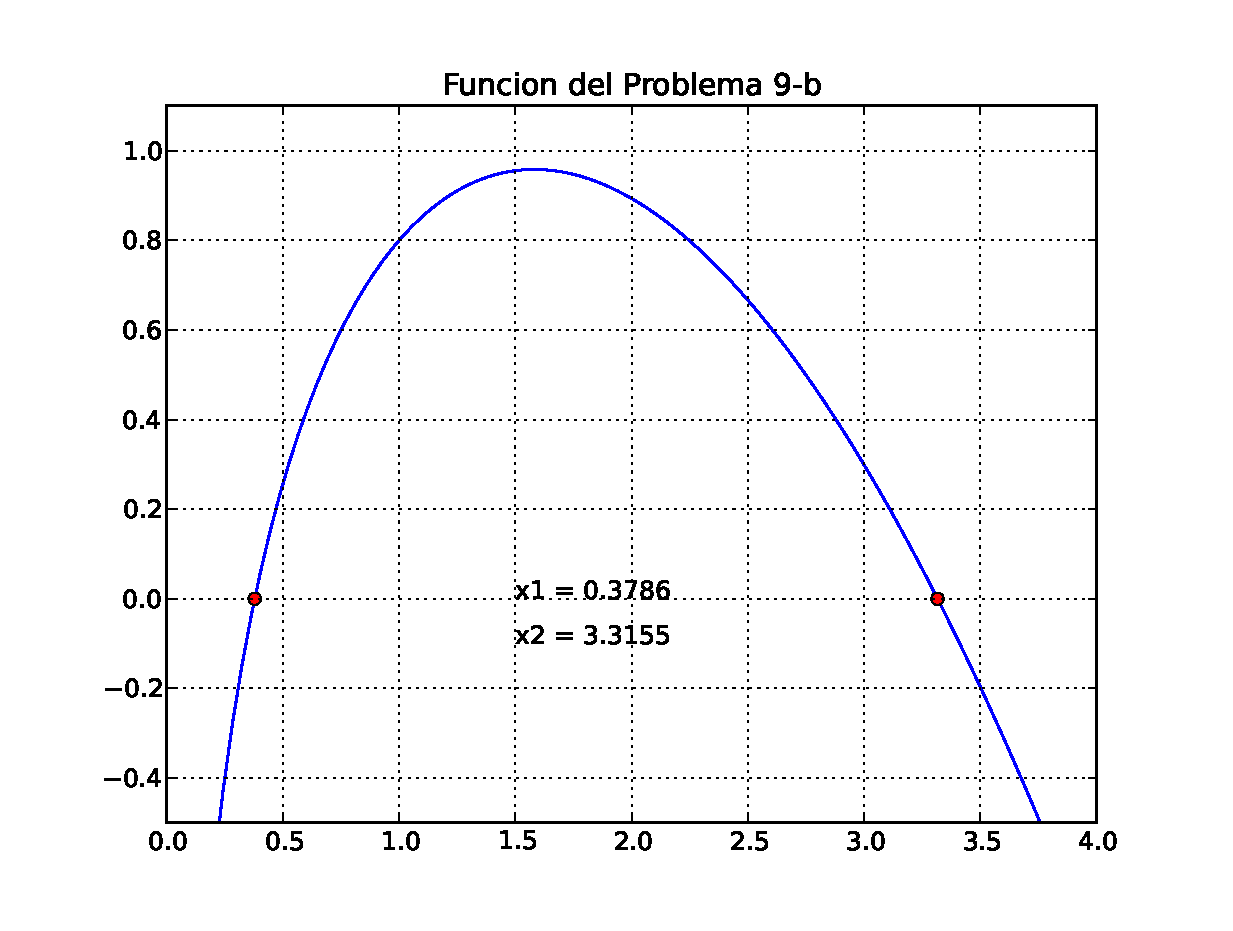
\includegraphics[scale=0.4]{Grafica9_b.eps} 
\end{figure}
\end{frame}
\begin{frame}
\frametitle{Inciso c)}
\begin{figure}
	\centering
	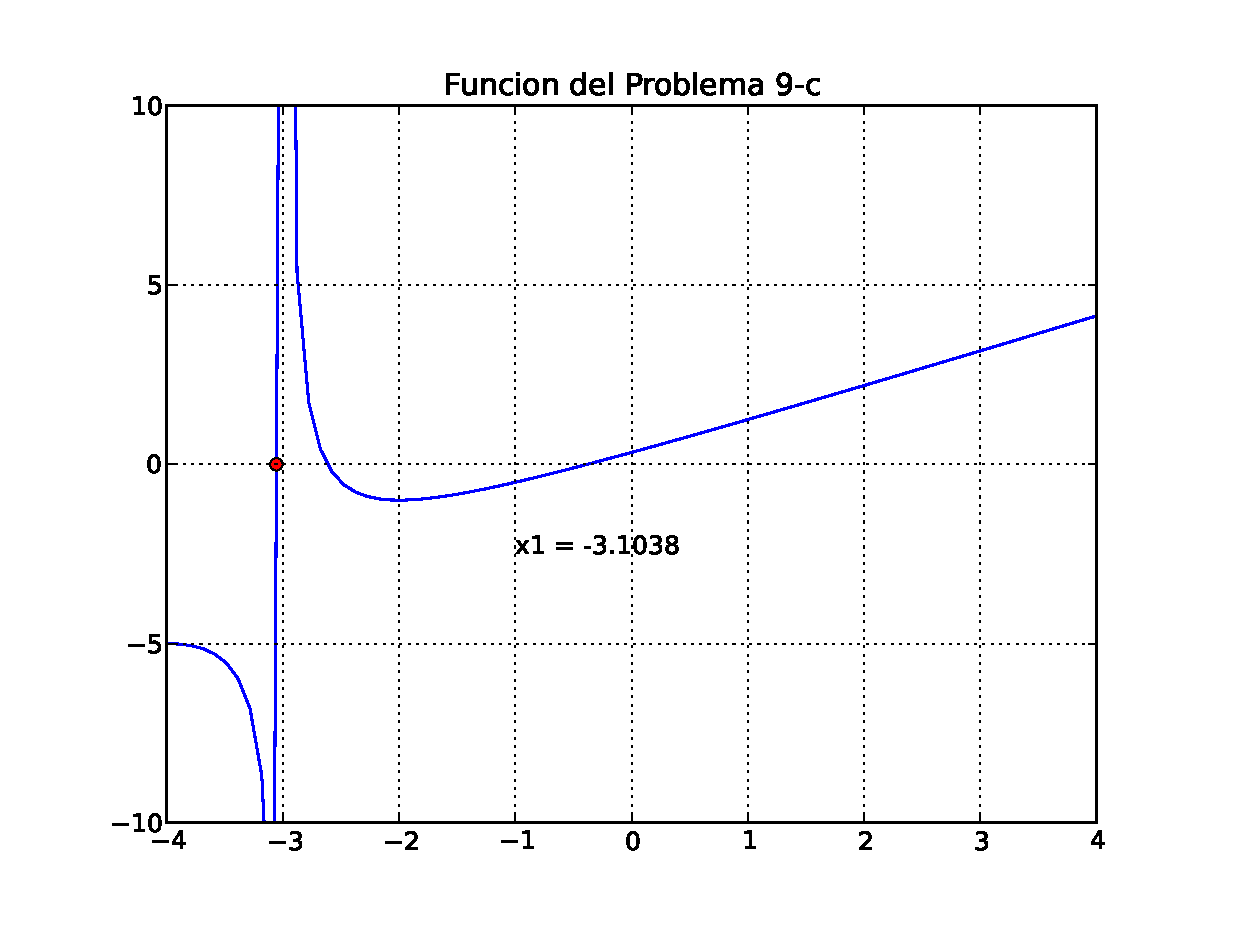
\includegraphics[scale=0.4]{Grafica9_c.eps} 
\end{figure}
\end{frame}
\end{document}